\chapter{واسط‌ها}

با توجه به معرفی اجزای جدید در معماری 
\lr{O-RAN}
این نیاز وجود دارد که برای ارتباط بین قسمت‌های مختلف، واسط‌های به صورت استاندارد تعریف شود تا بتوان برنامه‌های مختلفی توسعه داد و اجزای مختلف هم بتوانند به درستی با کمک این واسط‌های استاندارد شده با یک‌دیگر ارتباط برقرار کنند و دیگر همه چیز در اختیار فروشنده‌های قطعات نباشد.

در ادامه واسط‌های مختلفی که در شکل‌های فصل‌های مختلف دیدیم بررسی شده‌اند.

بعضی از این واسط‌ها توسط 
\lr{3GPP}
استاندارد شده‌اند که در 
\ref{fig:int1}
هم آورده شده‌اند. 

واسط
\lr{F1}
برای ارتباط بین
\lr{DU}
و
\lr{CU}
آماده شده است.

واسط
\lr{S1}
برای ارتباط بین
\lr{CU}
و هسته‌ی شبکه معرفی شده است.

\begin{figure}[H]
	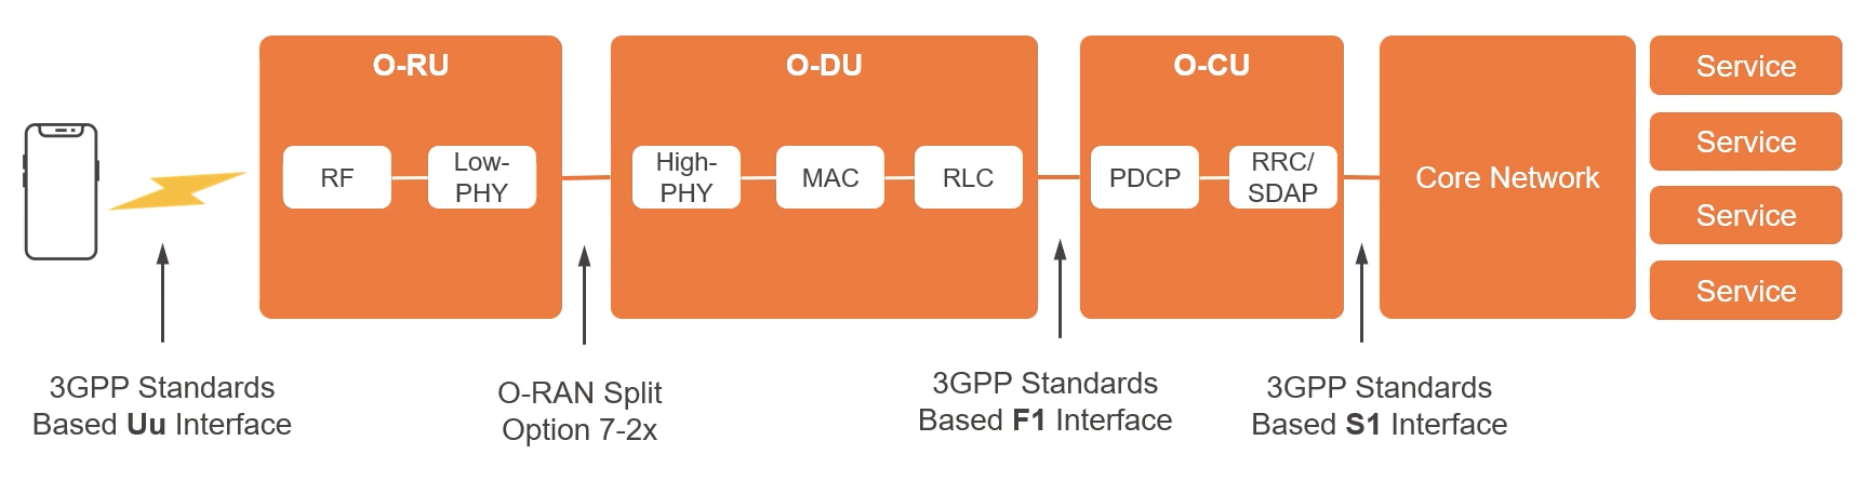
\includegraphics[width=0.85\columnwidth]{Picture/int1.png}
	\centering
	\caption{اجزای مختلف موجود در
		\lr{Near-Real-Time RIC}}
	\label{fig:int1}
\end{figure}

در ادامه در 
\ref{fig:int2}
به بررسی واسط‌های اختصاصی
\lr{O-RAN} 
پرداخته شده.

واسط
\lr{E2}
برای ارتباط بین
\lr{Near-Real-Time RIC}ها
با 
\lr{CU}
و
\lr{DU}
در نظر گرفته شده است.

واسط
\lr{A1}
برای ارتباط بین
\lr{Near-Real-Time RIC}
و 
\lr{None-Real-Time RIC}
 معرفی شده است.

واسط
\lr{O1}
برای ارتباط بین
\lr{SMO}
‌و اجزای مختلف اختصاصی 
\lr{O-RAN}
در نظر گرفته شده است.

\begin{figure}[H]
	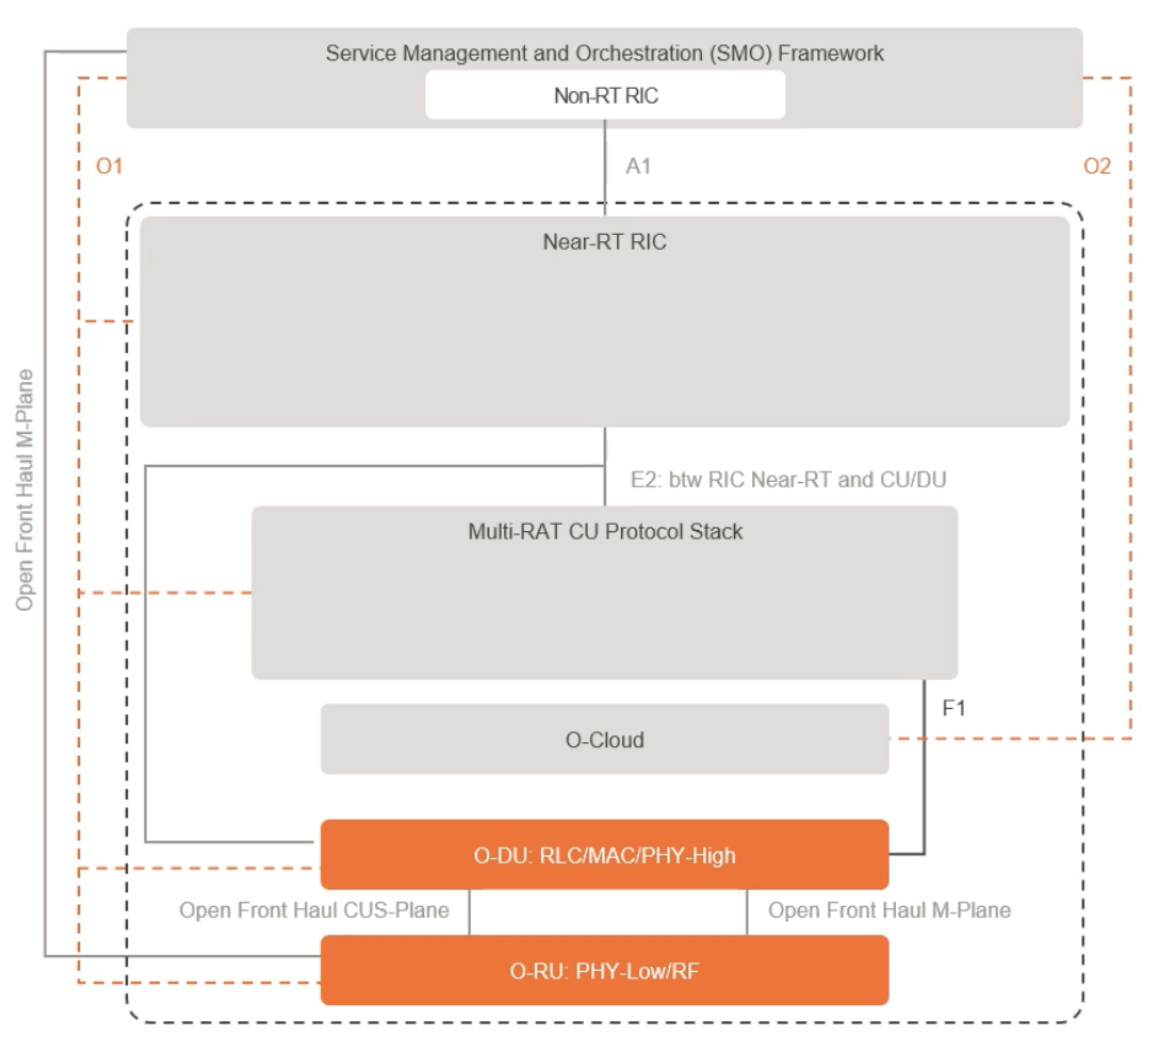
\includegraphics[width=0.85\columnwidth]{Picture/int2.png}
	\centering
	\caption{اجزای مختلف موجود در
		\lr{Near-Real-Time RIC}}
	\label{fig:int2}
\end{figure}